\chapter{Performance and Limitations}

It is important to know the capabilities of the airplane. It is also important to note how they change.

The Lance in particular has a huge variation in operating weight and center of gravity. A nose loaded, light Lance is practically a different airplane from a tail loaded, heavy Lance. It's important to explore the envelope of the plane in flight. But first, it's important to understand the envelope on the ground.


\section{The Power Curve}

We're engineers! We want a rigorous definition of all of the above speeds and their variation.

John S. Denker in ``See How It Flies'' has the most beautiful power curve diagram I've seen. It ties together the three major regimes of flight - normal, slow, and stalled - in one simple diagram. To me it is more clear than the classic diagram that plots lift, drag, and their ratio.

Here is Denker's power curve at idle power.

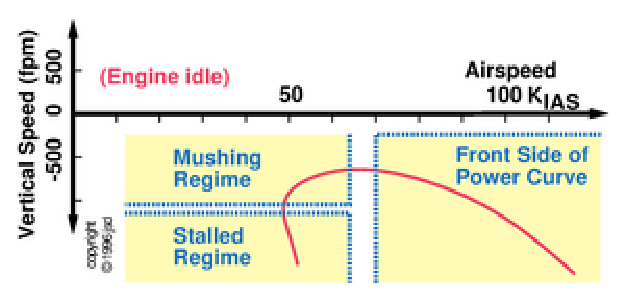
\includegraphics[width=\linewidth]{power-curve-regimes}

We plot airspeed on the X axis and vertical speed on the Y axis. The curve is decidedly not a function: it doubles back on itself. But we can piecewise define it as three functions. We draw a vertical tangent line on the left edge and a horizontal tangent line at the top edge. We'll talk about those tangent points later, they're important. But they define the limits of our three regimes of interest: normal, slow, and stalled. Or as Denker calls them, front side, mushing, and stalled.

Of course, this is at idle power. Since power makes us climb, but the power curve represents a fixed relationship between adjacent speeds that is always the same shape for the airplane, setting power moves the curve up or down. Denker wrote this for a fixed pitch prop, we can instead imagine 55, 65, and 75 percent power.

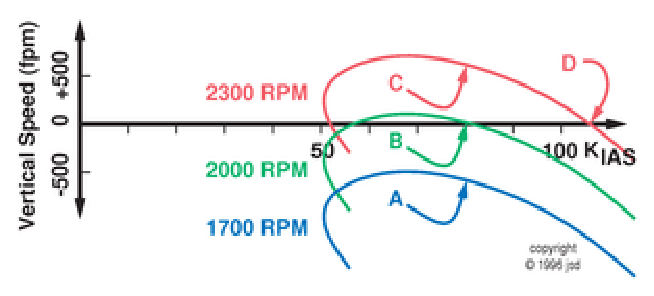
\includegraphics[width=\linewidth]{three-power}

The one gotcha with this explanation of the power curve is that it doesn't really explain what the flaps do directly. But we can derive it. Flaps change the shape of the airfoil and give us more lift in exchange for more drag. Low flap settings give us mostly more lift, high flap settings give us mostly more drag. More lift means moving the curve up. More drag meand moving the curve to the left.

\section{Speed Definitions}

Now that we've built a rigorous framework for describing airplane behavior using the power curve mode, we can go ahead and define some speeds. The following speeds are appropriate for a complex single engine airplane.

$V_S$ or $V_{S0}$ are the stalling speeds in the cruise or clean configuration: gear up, flaps up. This is the leftmost point on the power curve, the barrier between the stalled and mushing regimes.

$V_{S1}$ is the stalling speed in the landing or dirty configuration: gear down, flaps down. Since extending the flaps moves the power curve to the left, stalling speed is lowered.

$V_R$ is the rotation speed. Denker suggests a few knots below $V_Y$ unless specifically doing a short or soft field takeoff. In those cases I'd lift off right at or around $V_X$.

$V_X$ is the best \emph{angle} of climb speed, which we use to clear an obstacle. Denker draws a tangent from the origin of his performance curve axes to the power curve, the point of intersection is $V_X$. That speed will get slower if the power curve moves up (more lift) or to the left (more drag).

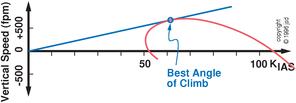
\includegraphics[width=\linewidth]{vx}

$V_Y$ is the best \emph{rate} of climb speed, which we use to gain altitude quickly. It corresponds to the maximum lift over drag speed, meaning, the most efficient point of operation. The maximum endurance speed is usually not far from this value. Denker draws this at the top of the power curve, or rather, where a horizontal line would be tangent to the curve. This does change with weight but as Denker points out the power curve is pretty flat here.

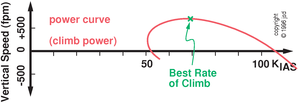
\includegraphics[width=\linewidth]{vy}

$V_G$ is the best glide speed. $V_Y$ is a reasonable guess.

$V_{FO}$ is the flap operation speed.

$V_{FE}$ is the flap extension speed.

$V_A$ is the maneuvering speed.

$V_{LO}$ is the landing gear operation (retraction) speed.

$V_{LE}$ is the landing gear extension speed.

$V_{NO}$ is the ``normal operating'' speed.

$V_{NE}$ is the never exceed speed.

\section{Lift and Weight}

Recall the lift equation:

\begin{equation}
L = \frac{1}{2} \rho V^2 C_L S
\end{equation}

, where $\rho$ is the density of the air, $V$ is velocity, $C_L$ is the coefficient of lift and $S$ is the surface area of the airfoil.

That $V^2$ term is key, Lift is proportional to the \emph{square} of velocity. So what happens if we halve the weight, and thus, the needed lift? Well, it would drop by the square root of a half, which happens to be $\frac{\sqrt{2}}{2} \approx 0.707\ldots$ which is about 29 percent. At three-quarters weight, it drops by the square root of three quarters, which is $\frac{\sqrt{3}}{2} \approx 0.866\ldots$ which is about 13 percent.

Denker points out that the entire power curve shifts up and to the right, with both power off and power on. He even points out a Cherokee Six as a specific example of this - how interesting!

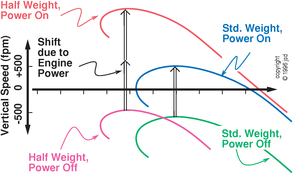
\includegraphics[width=\linewidth]{light-power}

The procedure to derive this curve is as follows:

\begin{enumerate}
\item Scale the entire standard weight, power off curve by the reduction factor. It will move up (since vertical speeds are chopped - a light airplane doesn't sink as much) and to the left (since airspeeds go down - a light airplane has a lower stalling speed).
\item Shift the curve up for power. Realize that, since the airplane is lighter, the curve will shift by a greater amount.
\end{enumerate}


\section{V Speeds for the Lance}

The Lance's POH defines a number of speeds. These speeds are commonly defined for single engine airplanes.

In this section, we explore the Lance's V speeds. For each V speed, we consider the definition of the speed, what it means operationally, and how it varies with respect to aircraft weight, aircraft loading (nose or tail heavy), density altitude, aircraft configuration (flaps, landing gear), and aircrat attitude.

\subsection{$V_{S}$ - Stalling Speed}


Recall the stalling speed variation formula:

\begin{equation}
V_S' = V_S \sqrt{\frac{New Weight}{Old Weight}}
\end{equation}


\begin{itemize}
\item Weight: a heavier airplane will require a higher angle of attack to fly and thus will have a higher stalling speed. A lighter airplane will have a lower stalling speed.
\item Loading: a nose heavy airplane will have a higher stalling speed due to the high angle of attack required to keep the nose flying. Conversely, an aft loaded airplane will have a lower stalling speed. But according to Denker the effect is relatively small.
\item Density Altitude: In thinner air, there is a greater discrepancy between indicated and calibrated airspeed. The airplane will stall at the same indicated airspeed but a higher true airspeed.  
\item Configuration: Changing the shape of the wings by deploying flaps changes the effective angle of attack. Deploying flaps will usually make the stall speed decrease.
\item Attitude: Stalling speed increases in a turn since we are using a larger component of our lift vector to keep the airplane aloft. In turbulence, the angle of incidence may vary, leading to an earlier stall because the relocation of the relative wind causes us to exceed critical angle of attack earlier. 
\end{itemize}


\begin{itemize}
\item Weight:
\item Loading:
\item Density Altitude:
\item Configuration:
\item Attitude:
\end{itemize}




